\chapter{Objekt Erkennung}

\section{Einführung}

Im Rahmen des autonomen Fahrens spielt die Objekterkennung eine bedeutende Rolle. Eine möglichst fehlerfrei agierende \ac{OD} bildet die Basis für das sichere Fortbewegen eines autonomen Fahrzeugs.
Hierbei kommen im industriellen Maßstab verschiedene Technologien zum Einsatz, vornehmlich die Erkennung anhand von Radar und / oder \ac{LiDAR} Sensor Daten, sowie die Klassifizierung von Kamerabildern.
Die \ac{LiDAR} und die Radar Erkennung basiert hierbei auf demselben Prinzip, nämlich die Reflektion von Laserstrahlen, bzw. Radarwellen, wodurch sich ein dreidimensionales Abbild der Umgebung darstellen lässt \cite[S.30f.]{Dr.Ing.ThomasTille.2018}.
Bis auf wenige Ausnahmen, wie Tesla, setzen alle Entwickler autonomer Fahrzeuge auf die \ac{LiDAR} Technologie als Ergänzung der Kameragestützen Erkennung \cite{AutoPilotReview.2019}.
Die Befürworter dieser Technologie sehen sie vor allem als Ergänzung der Kamera und Radarerkennung, während die Kritiker auf die hohen Preise der \ac{LiDAR} Sensoren verweisen, sowie auf annährend genau so hohe Erkennungsraten durch reine Kamera \ac{OD} \cite[S.8]{Wang.18.12.2018}.
Demzufolge können Kameras als Hauptwerkzeug für die \ac{OD} benutzt werden, wobei sie bei schwierigen Sichtverhältnissen (Schnee, Regen, etc.) von Radarsensoren unterstützt werden.
Im Rahmen dieses Projektes, bzw. dieser Arbeit wird mittels der Kamera \ac{OD} gearbeitet, wobei nur eine einzelne Kamera zum Einsatz kommt, was Auswirkungen auf die Distanz Berechnungen hat (siehe Kapitel \ref{sec:distance}).
Für die \ac{OD} verschiedener Objekte und Personen auf Bildern gibt es verschiedene Technolgien. Einige davon werden in Kapitel \ref{sec:comp} näher betrachtet, miteinander verglichen und bewertet, bevor sich Kapitel \ref{sec:yolo} mit der Implementierung des für diesen Projekt verwendeten Algorithmus, sowie Beobachtungen bei der Anwendung befasst. Abschließend wird in Kapitel \ref{sec:distance} dargelegt, wie die Distanz zu erkannten Objekten berechnet wird.

\section{Algorithmenvergleich}\label{sec:comp}

Die \ac{OD} setzt sich zusammen aus zwei Teilbereichen, die jeweils auch eigenständig funktionieren können, der \ac{OR} und daran anschließend die \ac{OC}. Die \ac{OC} ist dabei im Grundsatz eine Image Classification, also ein supervised Machine Learning Problem, bei dem Bilder verschiedener Objekte gelabelt und mithilfe eines \ac{CNN} erlernt werden \cite[S.615f.]{Manojkrishna.2018}. Die \ac{OR} hingegen soll visuell verdeutlichen wo sich erkannte Objekte im Bild befinden. Dies wird üblicherweise mithilfe farbcodierter Boxen, die um die einzelnen Objekte gelegt werden erreicht.

\subsection{Region-based Convolutional Networks}

Girshick et all stellten 2013 sogenannte \ac{R-CNN} zum Zwecke der Object Detction vor \cite{Girshick.2016} und beschreiben damit eine frühe Methode der effizienten \ac{OD}, die durch weitere Paper 2015 \cite{Girshick.30.04.2015} verbessert und 2016 \cite{Ren.04.06.2015} als Echtzeitalgorithmus angewendet wurden.

\begin{figure}[H]
    \centering
    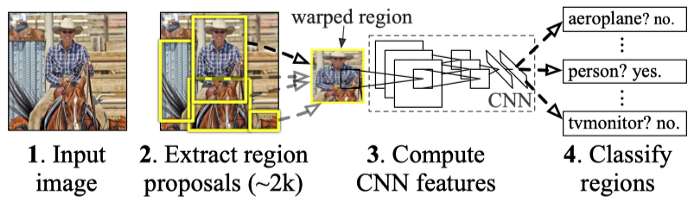
\includegraphics[scale=0.5]{./img/rcnn.png}
    \caption{R-CNN Aufbau, \cite[S.2]{Girshick.2016}}
    \label{fig:rcnn}
\end{figure}

Abbildung \ref{fig:rcnn} zeigt den Aufbau des zuerst beschriebenen \ac{R-CNN}. Hierbei greifen drei Module ineinander \cite[S.3-6]{Girshick.2016}. Die Aufgabe des ersten Moduls ist die Erzeugung von Region Proposals (dt. Region Vorschlag) für das Bild. Es sollen also die Regionen markiert, bzw. ausgegeben werden in dennen sich mögliche Objekte befinden. Hierfür wurde auf die Selective Search \cite{Uijlings.2013} zurückgegriffen. Die Autoren verweisen auf die Schwierigkeit mit Überlappungen, also dem sich nur teilweise in einer Region befindenden Objekt. Diese Probleme wurden durch das Einführen eines treshholds von 0.3 \cite[S.5]{Girshick.2016}. Alle Regionen, die unter diese Grenze fallen werden als negativ betrachtet und werden somit nicht weiter verarbeitet.
Auf den gefundenen Regionen aufbauend arbeitet nun ein \ac{CNN}, im speziellen eine Caffe Implementation desselben \cite{Jia.21.06.2014}. Die gewünschte Ausgabe dieses \ac{CNN}s ist ein Feature Vektor, der an das letzte Module, einer Anzahl \ac{SVM}, übergeben wird. Es handelt sich dabei um klassenspezifische \ac{SVM}, die im späteren Verlauf eine weitere Rolle übernehmen. Bei Erkennen eines Objekts wird durch den Output der \ac{SVM} eine klassenspezifische Bounding Box um das Objekt gelegt, um die genaue Lokalisierung zu verbessern \cite[S.12f.]{Girshick.2016}.
Wie bereits beschrieben wurde der ursprüngliche Ansatz der \ac{R-CNN} mehrfach verbessert, über das Fast \ac{R-CNN} \cite{Girshick.30.04.2015} hin zum Faster \ac{R-CNN} \cite{Ren.04.06.2015}. Diese zielen vornehmlich auf die schnellere Berechnung und Verarbeitung der Region Proposals, die den zeitaufwendigsten Schritt der \ac{OD} darstellt \cite[S.1]{Ren.04.06.2015}. Die Verarbeitungszeit wird bei Fast \ac{R-CNN} reduziert, indem nicht mehr für jede Region Proposal durchführen muss, es werden Berechnungen geteilt. Das \ac{CNN} nimmt als Input das Bild und alle Region Proposals und erzeugt darauf aufbauend eine Feature Map, die für die Erzeugung der Feature Vektoren benutzt wird. \cite[S.2f.]{Ren.04.06.2015}. Faster \ac{R-CNN} verbessert die Gesamtlaufzeit weiter, indem die Berechnungzeit der Region Proposals verringert wird. Hierfür werden Regional Proposal Networks genutzt, die als Ergänzung der bisher benutzten \ac{CNN} dienen können \cite[S.3f.]{Ren.04.06.2015}. Durch dieses Modul kann auf dem verwendeten Setup der Autoren eine \ac{OD} bei 5 \ac{FPS} durchegführt werden.

\subsection{Single Shot MultiBox Detector}

Trotz der erreichten Verbesserungen der \ac{R-CNN} erreichen diese dennoch keine zufriedenstellende Performance für Echtzeit \ac{OD}. Dies gelingt erst mit den YOLOv1 Netzwerken (siehe Kapitel \ref{sec:yolo-einführung}) und den \ac{SSD}. Letztere liefern eine etwa 74 prozentige Accuracy bei 59 \ac{FPS} \cite[S.2]{Liu.08.12.2015} und übertreffen damit Faster \ac{R-CNN} bei weitem, sowie YOLOv1. Diese Verbesserung wird erreicht, indem unter anderem auf die "bounding box proposals" \cite[S.2]{Liu.08.12.2015} verzichtet wird. Umgesetzt wird dies duch den Einsatz kleiner convolutional filter die Objektkategorien, und die dazu passenden bounding box locations, predicten. Die Filter werden auf verschiedenen Feature Maps im ganzen Verlauf des Netwerkes eingesetzt, so dass eine multipel skalierte Prediction erreicht wird \cite[S.2]{Liu.08.12.2015}.

\begin{figure}[H]
    \centering
    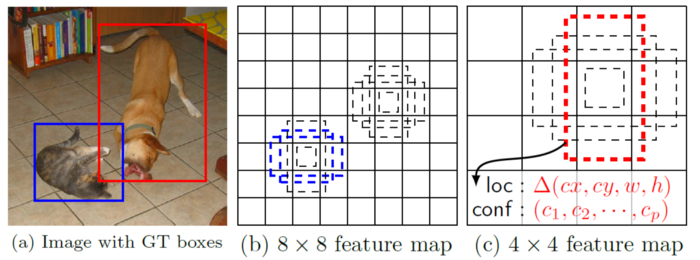
\includegraphics[scale=0.5]{./img/ssd.png}
    \caption{SSD framework, \cite[S.3]{Liu.08.12.2015}}
    \label{fig:ssd}
\end{figure}

Abbildung \ref{fig:ssd} zeigt ein Beispiel für die Bais Funktionsweise eines \ac{SSD}. Als Input wird ein Bild genommen auf dem Boxen für verschiedene Klassen (hier Hund und Katze) vermerkt sind. In Feature Maps mit verschiedenen Skalen (hier 8x8 und 4x4) sollen die Boxen des Bildes predicted werden. Dafür wird eine kleine Anzahl (hier 4) vordefinierter bounding boxen über das Bild gelegt und davon ausgehend predicted welche Klasse sich in ihr befindet, bzw. eine Anpassung der Dimensionen der Bounding Box vorgenommen \cite[S.3f.]{Liu.08.12.2015}.

\subsection{You Only Look Once}\label{sec:yolo-einführung}

Im Gegensatz zu herkömmlichen \ac{OD} Systemen verzichtet \ac{YOLO} auf langwierige Vorberechnungen, wie z.B. bei \ac{R-CNN} die Region Proposals. Das zuvor angesprochene \ac{SSD} arbeitet nach dem selben Prinzip, wurde jedoch erst nach der originalen YOLO Vorstellung beschrieben. Aus diesem Grund soll in diesem Kapitel zunächst auf die Basis Funktionsweise eines \ac{YOLO} Netzwerks eingegangen werden, bevor sich mit dem aktuellen (und für dieses Seminar verwendete) YOLOv3 beschäftigt wird.

\begin{figure}[H]
    \centering
    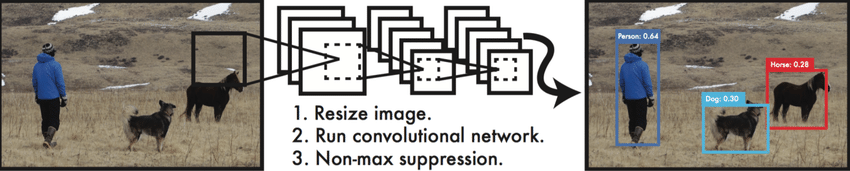
\includegraphics[scale=0.5]{./img/yolo.png}
    \caption{YOLO Detection System, \cite[S.1]{Redmon.08.06.2015}}
    \label{fig:yolo}
\end{figure}

Abbildung \ref{fig:yolo} zeigt dabei vereinfacht die Funktionsweise auf. Das Eingabebild wird auf eine vorgegebene Größe geändert, bevor in einem \ac{CNN} simultan verschiedene Bounding boxes, sowie die zugehörigen Klassenwahrscheinlichkeiten erzeugt werden \cite[S.1]{Redmon.08.06.2015}
\ac{YOLO} betrachtet dabei das Bild im Ganzen, womit auch kontextuelle Klasseninformationen in die \ac{OD} miteinbezogen werden können \cite[S.1f.]{Redmon.08.06.2015}. Dies unterscheidet es vom \ac{R-CNN}, das im Hintergrund mehr als doppelt so oft falsche Objekte erkennt als \ac{YOLO} \cite[S.2]{Redmon.08.06.2015}.
[Hier fehlt noch die genaue Funktionsweise des YOLO Netzwerks, sowie die Änderungen in YOLOv3 und warum sich für YOLO entschieden wurde]


\section{YOLO Implementierung}\label{sec:yolo}

\subsection{Vortrainierte Modelle}

Für die Implementierung der \ac{YOLO} \ac{OD} wurde auf vortrainierte config und weight Dateien zurückgegriffen. Redmon et all. stellen diese auf ihrer \href{https://pjreddie.com/darknet/yolo/}{Website} \cite{RedmonJosephFahradiAli.2020} zur Verfügung.
Für diese Arbeit wurde YOLOv3, sowie YOLOv3-tiny verwendet.
In der dieser Arbeit beigefügtem Git Repository befindet sich die \ac{OD} in der Datei /AutonomousCar/main/object-detectiion/object-detection.py. In der nun folgenden Erklärung werden kurze Code Abschnitte verwendet, für eine komplette Durchsicht des Codes sei auf die oben genannte Datei verwiesen.
Die Implementierung basiert dabei auf Tutorials von Adakane \cite{DarshanAdakane.2019, DarshanAdakane.2019b}.
Die vortrainierten weights / cfgs basieren auf den coco Datensatz (Z. 10). Wie bereits in Kapitel \ref{sec:yolo-einführung} dargelegt wird das Image auf eine bestimmte Größe, hier 416x416 skaliert (Z.3). Unser Code bietet die Möglichkeit (Zeile 7) zwischen den verschiedenen YOLO verisonen zu wechseln, was aufgrund der Performance auf dem Rapsberry Pi nötig ist. Auf diesen Punkt wird in Kapitel \ref{sec:performance} eingegangen. In Zeile 13 und 14 wird das vorverarbeitete Bild dem Netwerk übergeben. Als Rückgabe wird eine Liste der erkannten Objekte erwartet.

\begin{lstlisting}[language=Python]
...
# preprocess image
blob = cv2.dnn.blobFromImage(img_original, 1 / 255.0, (416, 416), 
swapRB=True, crop=False)

# load network
output_layers, net = load_yolo(tiny=tiny)

# load coco list
class_list = load_coco_names()

# detect objects
net.setInput(blob)
outs = net.forward(output_layers)
...
\end{lstlisting}

Diese Ergebnisse werden dann in zwei Funktionen (information-cal und information-draw) weiter verarbeitet. Information-cal (Datei ab Zeile 68), überprüft dabei für jedes Objekt in outs, ob es mit einer zufriedenstellenden Confidence (hier 0.5) erkannt wurde. Außerdem werden die Höhe, Breite, x- und y-Position der Bounding Box berechnet und gespeichert. Diese Box wird außerdem mit dem Objekt-Namen angereichert.
Daraufhin werden die Ergebnise der information-draw Funktion übergeben, die dann mithilfe von opencv in das Eingabebild eingezeichnet werden. opencv bietet dabei die Möglichkeit das Schriftbild zu verändern.

\begin{lstlisting}[language=Python]
...
for i in range(len(boxes)):

    if i in indexes:
    
        x, y, w, h = boxes[i]
        label = str(class_list[class_ids[i]])
        full_label = label + ", " + str(round(confidences[i] * 100, 2))
        color = colors[class_ids[i]]
        cv2.rectangle(img, (x, y), (x + w, y + h), color, rec_width)
        cv2.putText(img, full_label, (x, y -5), font, txt_height,
        color, text_width)
...
\end{lstlisting}

Das oben gezeigte beschreibt die Erkennung für jeweils ein Bild. Dies kann auf einen Videostream (z.B. Webcam, hier Pi-Camera) umgeschrieben werden, indem jeder einzelne der von der Kamera aufgezeichneten Frames diesen Prozess durchläuft.

\subsection{Individuell trainiertes Modell}

Aufgrund des Modellmaßstabes des Projekts wird das Auto auf keine Menschen treffen, die die \ac{OD} auslösen können.
Aus diesem Grund wurde versucht ein individuelles \ac{YOLO} Netzwerk zu trainieren, dass Playmobilmenschen erkennt. Im Folgenden sollen die dafür verwendeten Schritte beschrieben werden.
\begin{enumerate}
    \item Datenbeschaffung:
    Als Datenquelle wurde zunächst die PlaymoDB \cite{PlaymoDB.2020} nach passenden Bildern durchsucht. Abbild \ref{fig:playmo} zeigt ein Beispielbild. Hieran wird auch ein mögliches Hemmniss deutlich. Der überwiegende Teil der Bilder ist aus diesem Winkel und dieser Position aufgenommen worden, sodass fraglich bleibt wie gut das Training funktioniert.
    
    \begin{figure}[H]
        \centering
        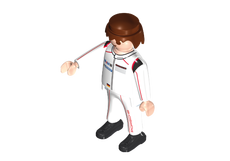
\includegraphics[scale=0.5]{./img/playmo.jpg}
        \caption{PlaymoDB Bild}
        \label{fig:playmo}
        \\ Quelle: https://playmodb.org/cgi-bin/showpart.pl?partnum=302000200404
    \end{figure}
    
    Alternativ dazu wurden eigene Bilder (im Github Repositorry unter ...) verwendet.
    \item Labeling:
    Ein zentraler (und zeitaufwendiger) Punkt des Trainings ist das Labeling der zuvro beschafften Bilder. Dieses geschieht in unserem Fall über das pip labeling Tool labelImg (siehe Abbildung \ref{fig:label}. Hierbei werden die Objekte (Playmobilfiguren) mit einer passenden Bounding Box versehen. Diese Informationen werden in einer txt Datei gespeichert im Format <ClassID> <x-Zentrum> <y-Zentrum> <Breite> <Höhe>.
    
    \begin{figure}[H]
    \centering
    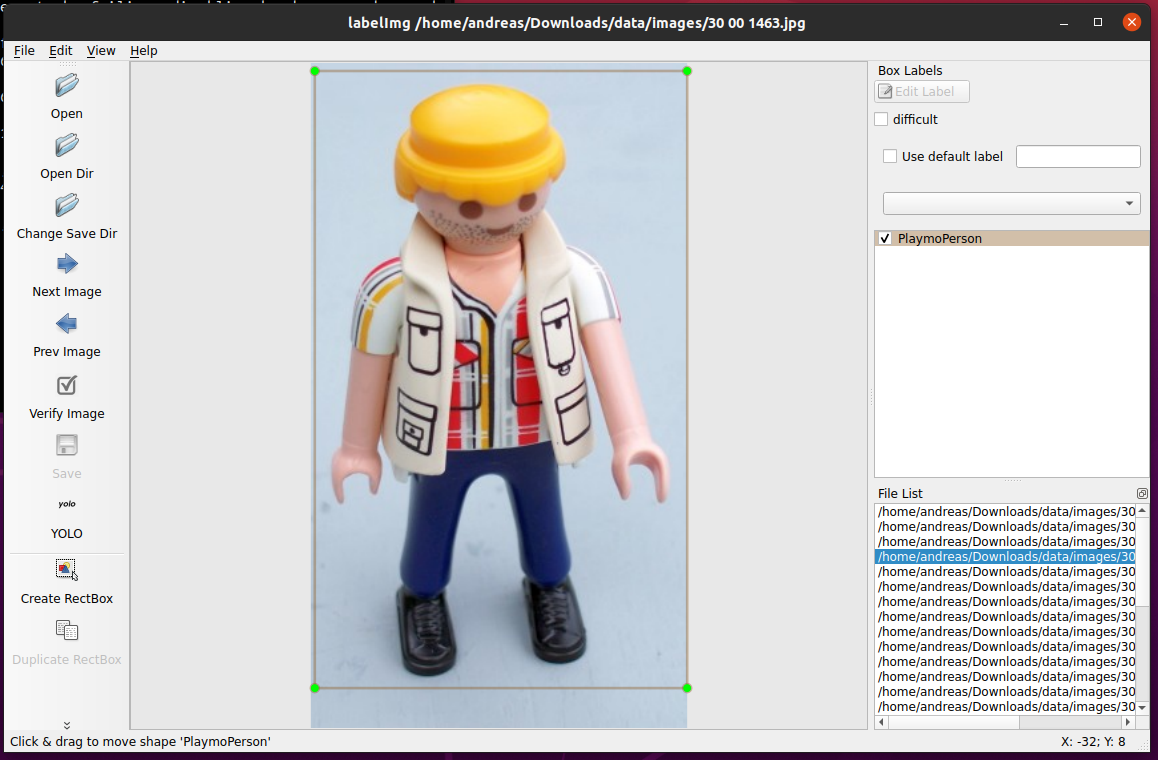
\includegraphics[scale=0.2]{./img/label.PNG}
    \caption{LabelImg Anwendung}
    \label{fig:label}
    \end{figure}
    
    \end{enumerate}
    \item Training:
    Für das Training wird auf ein Tutorial, sowie ein bereitgestelltes Google Colab Notebook zurückgegriffen \cite{Rafi.2019}. Erwähnt seien die nötigen Anpassungen in den cfg Dateien (ob \ac{YOLO} oder tiny \ac{YOLO}). Hierfür müssen in den YOLO Layern, sowie dem jeweils vorgelagerten Conv Layer Veränderungen vorgenommen werden.
    \begin{lstlisting}
    ...
    [convolutional]
    size=1
    stride=1
    pad=1
    filters=18
    activation=linear
    
    [yolo]
    mask = 3,4,5
    anchors= 5.80289956, 11.72601733, 7.61052314, 11.16109429, 11.2596055, 12.61, 11.698908, 12.6685, 12.263004, 12.584, 12.816258, 12.038
    classes = 1
    num = 6
    jitter=.3
    ignore_thresh = .7
    truth_thresh = 1
    random=1
    ...
    \end{lstlisting}
    Diese betreffen die filters in Zeile 6, diese müssen entsprechend der Formel,
    \begin{equation}
        filters = (Klassenanzahl+5) * num / 2
    \end{equation}
    also: filters = (1+5)* 6/2 = 6*3 = 18, gesetzt werden.
    Außerdem muss in Zeile 12 die Anzahl der Klassen angepasst werden.
    Nach diesen Anpassungen kann das Colab Notebook ausgeführt werden, welches nach einer definierten Anzahl an Trainingsschritten die Gewichte ausgibt.

\subsection{Performance}\label{sec:performance}

[Über Performance von normalen und tiny yolo schreiben]

\section{Distanz Errechnung}\label{sec:distance}

Mithilfe von OpenCV ist es möglich den Abstand zu einem erkannten Objekt in einem Bild relativ zur Kamera zu messen.
Hierfür wird auf ein Tutorial von Rosebrock zurückgegriffen \cite{AdrianRosebrock.2015}.
Die Berechnungen basieren auf der Dreiecks Ähnlichkeit (triangle similarity). Diese besagt in unserem Fall im Groben, dass wir ausgehend von einem Objekt in einem Foto, dessen Weite und Abstand bekannt sind, die Brennweite (focal length) berechnet werden kann. VOn dieser ausgehend kann dann für ein neues Objekt, dessen Pixelweite bekannt ist, der Abstand zur Kamera berechnet werden. Das neue Objekt, bzw. die neue Breite sind im Fall dieses Projektes die Weite der Bounding Box eines bestimmten Objekts.
Für dieses Modell wurde als Kalibrierungsmaßstab eine Soundbox mit 16cm Breite und einem 50cm Abstand zur Kamera gewählt. Mithilfe des in Kapitel \ref{sec:greyscaling} beschriebenen Grayscalings, sowie einer opencv Funktion, die es erlaubt Konturen zu finden und zu extrahieren (cv2.findContours()) kann die Pixelweite der Soundbox extrahiert werden.

\begin{figure}[H]
    \centering
    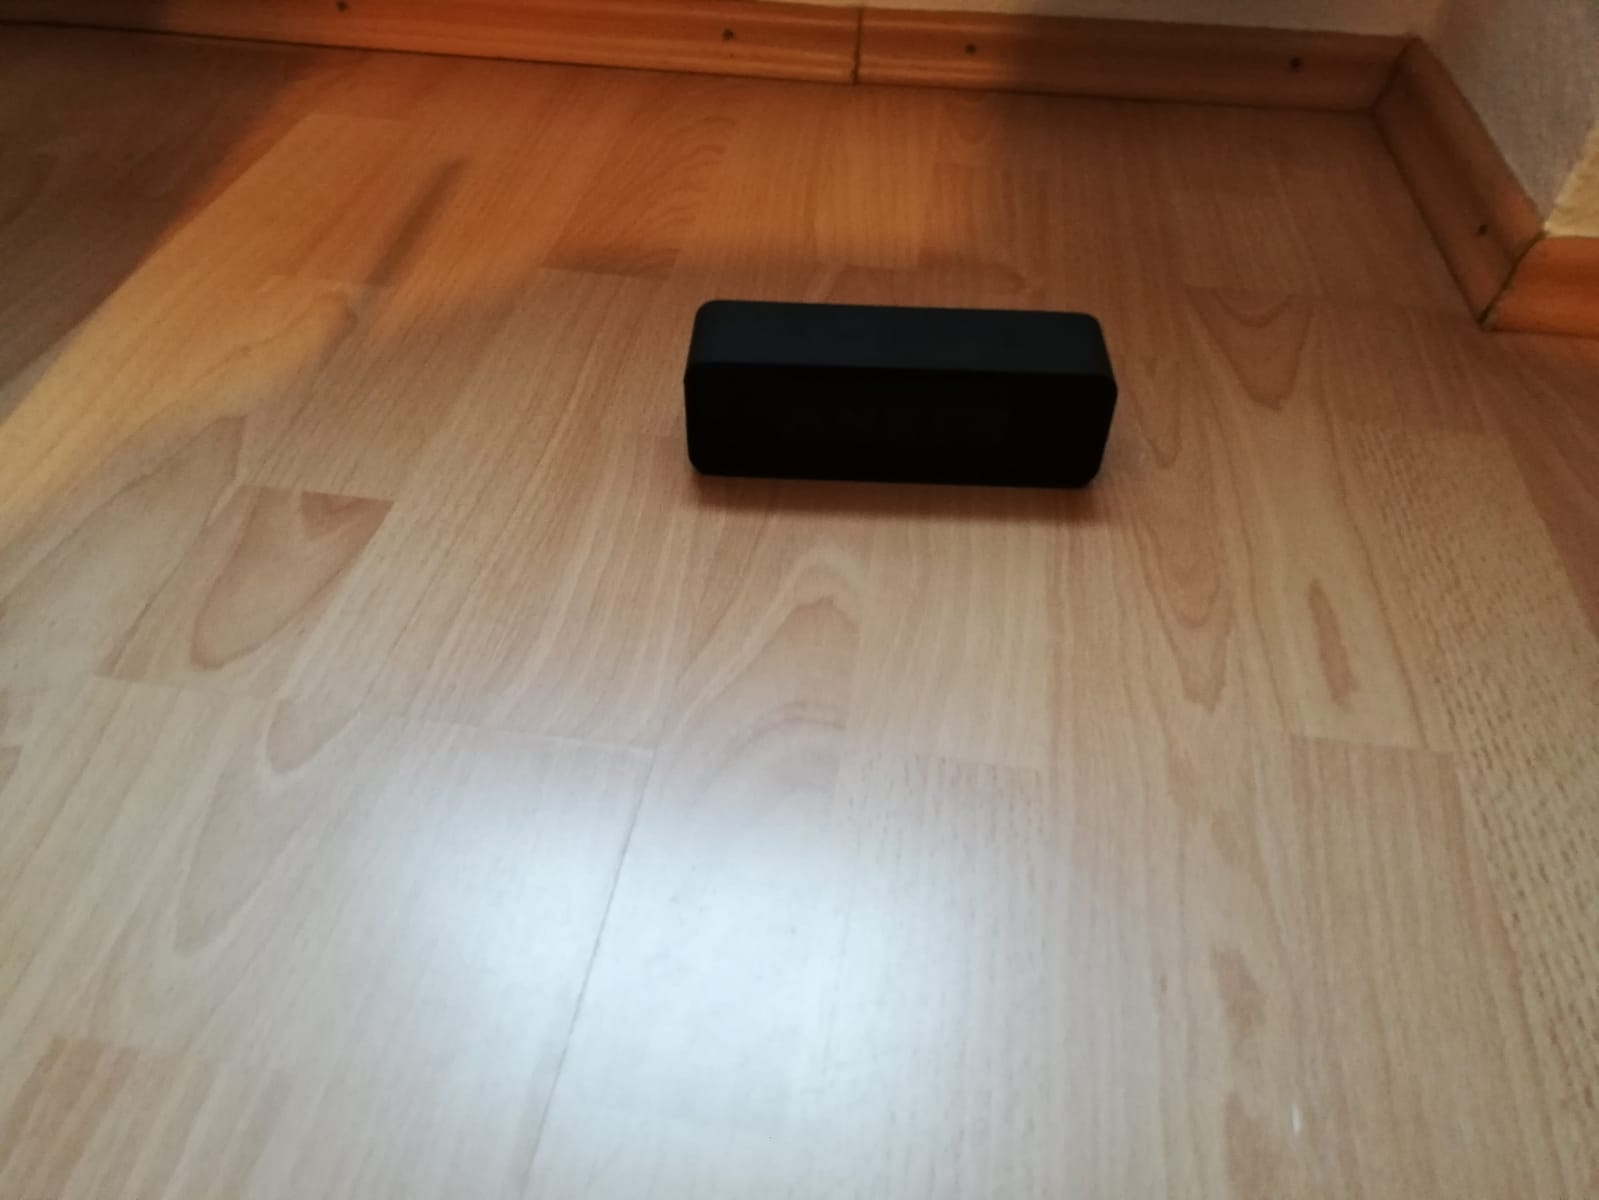
\includegraphics[scale=0.1]{./img/marker.jpg}
    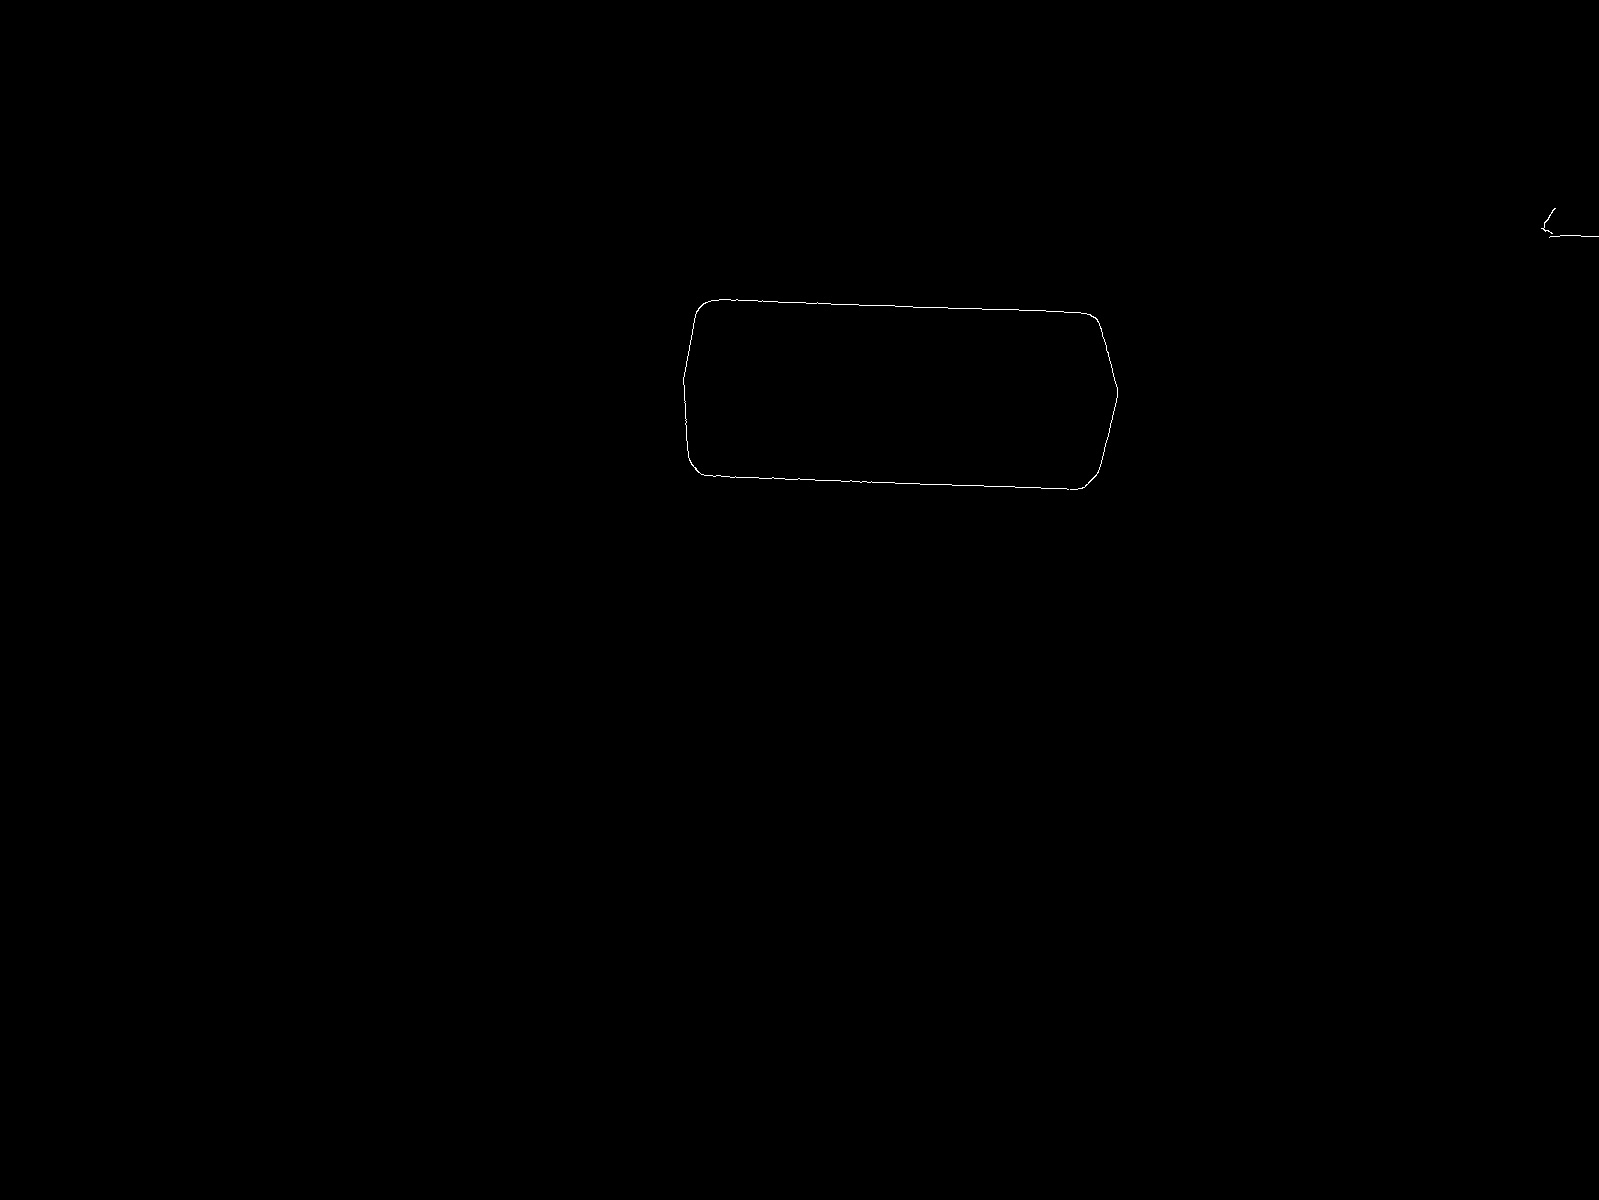
\includegraphics[scale=0.1]{./img/marker_gray.jpg}
    \caption{Marker (Original links, Kontur rechts)}
    \label{fig:marker}
\end{figure}

Die focal length errechnet sich durch:
\begin{equation}
    focalLength = (marker-pixel-width * marker-distance) / marker-width
    \label{equ:focalLength}
\end{equation}

Hiervin ausgehend kann die Distanze zu Objekten errechnet werden:
\begin{equation}
    distance = (marker-width * focalLength) / object-width
    \label{equ:distance}
\end{equation}

Zu beachten ist, dass die focal Length kamera, sowie Winkelspezifisch ist. Es ist somit auf ein aktuelles Kalibrierungsfoto zu achten.

In unserem Projekt soll mithilfe der Distanz Messung ein Call to Action erreicht werden. In der zugehörigen Funktion check-reation (Z. 106) wird in einer List festgelegt bei welchen Klassen die Distanz gemessen werden soll, z.B. person. Sobald eine Person erkannt wird, wird für diese auch laufend die Distanz errechnet. Im folgenden kann dann an das Auto ausgegeben werden zu stoppen, falls sich eine Person unterhalb eines bestimmten Abstands zur Kamera (und damit zum Auto) befindet.